\chapter{Analysen und Nutzertests} \ref{sec:analysisTests}
Dieses Kapitel behandelt das Entwerfen und die Durchführung von Experten- und Nutzertests zum Feststellen schwerwiegender User-Experience-Probleme. Dazu wird zunächst ein Testkonzept erstellt, das sich in Experten und Nutzertests aufteilt. Anhand dieses Konzeptes werden die Analysen (Expertentests) durchgeführt und anschließend die Nutzertests, für die zufällige Testpersonen ausgewählt werden. Die Ergebnisse der Tests werden abschließend ausgewertet um im nächsten Kapitel als konkrete Probleme behandelt zu werden.\par
\section{Entwicklung des Analyse-/Testkonzepts} \label{sec:analysisConcept}
Die Entwicklung des Testkonzeptes orientiert sich an den durch Ullenboom vorgegebenen Richtlinien zum Ablauf eines Testvorganges (siehe Kapitel \ref{sec:methods}).\par
\subsection{Festlegen von Ziel und Zweck}
Das Ziel der Untersuchung ist das Aufdecken von gravierenden Problemen bei der Bedienung der Anwendung. Dabei geht es um Probleme, welche die 5 Kernaspekte der Usability (siehe Kapitel \ref{sec:usability}) beeinträchtigen und ein positives Nutzungsempfinden schmälern oder unter Umständen schmälern könnten.\par
Der Gegenstand der Untersuchung ist die Client-Software FalkoFX. Die Analysen sind auf die Bereiche beschränkt, die bereits fertig implementiert sind. Dies sind die 4 verschiedenen Anwendungsfälle, die im ersten Reiter der Navigationsleiste zu finden sind und die anwendungsspezifischen Einstellungen des letzten Reiters der Navigationsleiste. Nur der Versionsvergleich, der unter dem zweiten Reiter zu finden ist, ist von der Untersuchung ausgeschlossen.\par%Um die Testergebnisse nicht zu beeinflussen, wird dieser vorab aus der Navigationsleiste entfernt.
%\heading{Untersuchungsdesign und Auswahl der Testverfahren}
\subsection{Untersuchungsdesign}
In diesem Schritt werden die Testverfahren für Experten- und Nutzertests ausgewählt. Anschließend werden Testszenarien entworfen, die eine möglichst große Abdeckung der Funktionalitäten von FalkoFX erlauben.\par
\heading{Auswahl der Testverfahren}
Sowohl für die Experten- als auch für die Nutzertests kommen verschiedene Arten von Tests in Frage. Einige lassen sich jedoch initial ausschließen, da sie dem Ziel der Tests nicht dienlich sind. Dazu zählen das Hallway-Testing, KLM/GOMS und der A/B-Test. Das Hallway-Testing eignet sich nur für kurzfristige Tests einer kleinen Funktionalität während der Implementierungsphase, nicht jedoch für das Gesamtheitliche Testen einer Anwendung. Die KLM/GOMS-Analyse hilft dabei, die Effizienz eines Softwareproduktes zu beurteilen, zeigt aber nicht auf, an welchen Stellen Handlungsbedarf besteht bzw. wo explizite Probleme vorliegen. Der A/B-Test ist ein vergleichender Test. Es wäre durchaus möglich, im Rahmen des Tests FalkoFX mit dem originalen Falko-Client zu vergleichen, um die Verbesserung des Nutzungsverhalten nachzuweisen, aber auch dies ist nicht zweckdienlich. Auf diese Weise würde nahezu doppelter Aufwand zur Feststellung von Nutzungsproblemen im FalkoFX-Client betrieben werden.\par
Unter den Expertentests ist die Heuristische Evaluation ein geeignetes Verfahren. Die definierten Heuristiken, nach denen Anwendungen bewertet werden können, bieten dem Tester vorgefertigte Kriterien, von denen er sich leiten lassen kann. Der Aufwand des Tests ist nicht allzu hoch und doch werden zuverlässige Ergebnisse erzielt. Der Cognitive Walkthrough, der ebenfalls ein Expertentestverfahren darstellt, ist ebenfalls nicht sehr aufwendig, erfordert aber ein hohes Maß an Verständnis für die Arbeitsabläufe des Endanwenders. Ist dieses nicht gegeben, können schnell falsche Annahmen getroffen und die Ergebnisse verfälscht werden. Da dieses Wissen über die internen Arbeitsabläufe beim Kunden nicht in ausreichendem Maße gegeben ist, wird von dieser Methode Abstand genommen. Dementsprechend wird nur die Heuristische Evaluation im Rahmen der Expertentests durchgeführt.\par
Im Bereich der Nutzertests stehen noch der Usability Walkthrough, der Formale Usability-Test und die Usability-Befragung zur Verfügung. Der Usability Walkthrough ist eine Methode, die vermehrt im frühen Entwicklungsstadium einer Anwendung zum Einsatz kommt, da es hier vor allem darum geht, einzelne, komplexe Handlungsschritte zu testen. Das Ziel der Tests ist es jedoch nicht, einzelne Schritte zu testen, sondern einen Überblick über die gravierendsten Probleme zu erhalten. Ein Usability Walkthrough mit den erdenklichen Szenarien wäre ein unverhältnismäßig hoher Aufwand. Für den Anwendungsfall eher geeignet ist der Formale Usability-Test in Kombination mit der \textit{Thinking Aloud}-Methode und einer Eye-Tracking-Analyse. Ergänzend kann eine Usability-Befragung unter Zuhilfenahme vorgefertigter Fragebögen durchgeführt werden. Die Durchführung einer solchen Befragung bei einer eingeschränkten Testnutzerzahl erfordert keinen großen Mehraufwand.\par
\heading{Entwurf Heuristische Evaluation}
\editHere{Reference Heuristik}
Die Heuristische Evaluation wird anhand der Heuristik von Nielsen und Molich durchgeführt, die 10 Prinzipien beinhalten.\editHere{Source} Zunächst werden möglichst realitätsnahe Aufgabenstellungen definiert, welche den Großteil der durchzuführenden Aktivitäten abdecken. Bei jedem Schritt dieser Aufgaben wird untersucht, ob alle Prinzipien erfüllt werden. Ist dies nicht der Fall, liegt möglicherweise ein Usability-Problem vor.\par
\editHere{Die Aufgabenstellungen sind im Anhang zu finden}\par
\heading{Entwurf Formaler Usability-Test}
Für den Formalen Usablity-Test wird ein Testsystem benötigt. Dies beinhaltet die Hardware (Computer, Ein- und Ausgabegeräte), die lauffähige Software nach dem aktuellen Entwicklungsstand und das konfigurierte Eye-Tracking-System mit Softwareunterstützung für die Aufzeichnung und Analyse von Eye-Tracking-Daten.%Funktionen der Software, die nicht voll funktionsfähig sind, werden außen vor gelassen.
\par
Die Auswahl der 5 Testkandidaten erfolgt firmenintern. Die Tatsache, dass alle Testkandidaten einen informationstechnischen beruflichen Hintergrund besitzen, könnte sich sowohl vorteilhaft als auch nachteilhaft auf die Testergebnisse auswirken. Eine positive Beeinflussung könnte dadurch erfolgen, dass die Kandidaten sicherer im Umgang mit der unbekannten Anwendung sind. Die \enquote{Angst} Fehler zu begehen ist aufgrund des technischen Wissens möglicherweise geringer. Andererseits würde ein tatsächlicher Endanwender, der zuvor mit dem produktiven Falko-System gearbeitet hat, zu einem gewissen Maße unterschiedlich agieren, da die Erfahrung und so auch die Erwartungshaltung eine andere ist.\par
Die Art der Aufgabenstellung, welche die Nutzer zu erfüllen haben, ist weniger abstrakt formuliert als es bei Produkttests üblich ist. Dies soll für eine Kompensation der Erfahrungsdifferenzen zu den tatsächlichen Endanwendern und der Defizite an fachlichem Wissen, das für die Bedienung von Vorteil wäre, sorgen. Dennoch werden durch die Aufgabentexte keine Hinweise auf den Lösungsweg gegeben. Diese muss sich der Anwender selbst erschließen. Die Testfälle orientieren sich an denen der Heuristischen Evaluation, sind aber weniger umfangreich.\par
\editHere{Das Testkonzept ist im Anhang zu finden}\par
\heading{Entwurf Usability-Befragung}
Der Aufwand für die Usability-Befragung wird so gering wie möglich gehalten. Sie dient vor allem dem Ziel, im Rahmen einer Einzelauswertung, weitergehende Informationen über den Begeisterungsfaktor der Software zu erlangen. Aus diesem Grund wird ein vorgefertigter Fragebogen genutzt. Es wurde sich hier für die Kurzform des einfach zu handhabenden Fragebogens \enquote{AttrakDiff} entschieden, der neben der pragmatischen Qualität auch die hedonische Qualität (Freude an der Verwendung) berücksichtigt. Dadurch wird die User Experience stärker in den Fokus der Befragung gerückt, anstatt nur die Usability.\editHere{Cite}\par
Nach Beendigung des Formalen Usability-Tests erhält der Testkandidat den Fragebogen, der \editHere{X} subjektiv empfundene Eigenschaften der Anwendung aufzählt, die jeweils auf einer 7 stufigen Skala bewertet werden. Ein Beispiel für eine solche Eigenschaft ist die Schönheit der Anwendung.\par
\editHere{Der Fragebogen ist im Anhang beigefügt.}
\section{Durchführung der Analysen} \label{sec:analysisExecution}
An dieser Stelle wird nur exemplarisch der Arbeitsablauf für die erste Aufgabenstellung der Heuristischen Evaluation aufgeführt. Alle gefundenen Probleme werden jedoch in Abschnitt \ref{sec:analysisConclusion} dargelegt und aufgegriffen. Es werden alle Prinzipien der Heuristik bei jedem Schritt versucht zu beantworten, um eine Vorstellung der nötigen Schritte zu vermitteln. Für die Auswertung relevant sind schlussendlich jedoch nur die Prinzipien, die in einem Schritt nicht erfüllt werden.\par
\textbf{Fragestellung:} Welche Länder werden als Höhenland eingestuft?\par
\textbf{Schritt 1:} Auswählen des Anwendungsfalles \enquote{Land}
\begin{enumerate}
 \item \textit{Ist der Systemstatus sichtbar?} Ja, eine Ladeanimation signalisiert dem Nutzer, dass während des Bildschirmwechsels Daten geladen werden müssen.
 \item \textit{Stimmen System und reale Welt überein?} Ja, das System ist nach den Arbeitsabläufen des Kunden in 4 verschiedene Anwendungsfälle gegliedert.
 \item \textit{Hat der Nutzer genügend Kontrolle und Freiheit?} Ja, durch die Markierung in der Navigationsleiste wird deutlich, welche Aktionen der Nutzer ausführen kann und welche gerade nicht verfügbar sind. Für die Navigation momentan nicht relevante Informationen sind ausgeblendet (z.B. Seitenleiste).
 \item \textit{Ist die Lösung konsistent und hält Standards ein?} Ja
 \item \textit{Wird versucht Fehler zu vermeiden?} Ja, nicht bedienbare Elemente, die zu einem invaliden Zustand führen würden, sind deaktiviert (bspw. Seitenleiste).
 \item \textit{Wird Erkennen Erinnern vorgezogen?} Ja, die Piktogramme der Navigationselemente sind sprechend und unterschiedlich gestaltet. Zusätzlich erscheinen Tooltips über den Schaltflächen.
 \item \textit{Sind Abläufe flexibel und effizient?} Ja, Mnemonics unterstützend den Nutzer für den direkten Zugriff auf Funktionen.
 \item \textit{Ist das Design ästhetisch und minimalistisch?} Ja, es sind nur die Navigationselemente sichtbar, zu denen direkt navigiert werden kann. Unterpunkte von Navigationselementen sind ausgeblendet.
 \item \textit{Gibt es Unterstützung bei Fehlern?} Bislang keine Fehlerquelle vorhanden
 \item \textit{Sind Hilfe und Dokumentation vorhanden?} Ja, es existieren Hilfetexte im Navigationsbereich. 
\end{enumerate}
\textbf{Schritt 2:} Auswählen des Attributes \enquote{Höhenland} für die Filterung
\begin{enumerate}
 \item \textit{Ist der Systemstatus sichtbar?} Ja, Änderungen werden umgehend sichtbar. Die angewählte Kategorie wird jeweils hervorgehoben. Nach der Auswahl eines Filterattributes wird dieses entfernt und ist sofort in der Liste der ausgewählten Attribute zu finden.
 \item \textit{Stimmen System und reale Welt überein?} Ja, die auswählbaren Eigenschaften entsprechen den tatsächlichen Gegebenheiten, die der Nutzer aus seiner täglichen Arbeit gewohnt ist.
 \item \textit{Hat der Nutzer genügend Kontrolle und Freiheit?} Ja, der Nutzer kann frei durch die verschiedenen Kategorien navigieren und auf einfache Weise Eigenschaften an- und abwählen.
 \item \textit{Ist die Lösung konsistent und hält Standards ein?} Standards werden eingehalten. Im Gegensatz zu der Navigationsleiste sind hier keine Tooltips für die Piktogramme vorhanden.
 \item \textit{Wird versucht Fehler zu vermeiden?} Nicht anwählbare Funktionen sind deaktiviert.
 \item \textit{Wird Erkennen Erinnern vorgezogen?} Die auswählbaren Kategorien sind mit sprechenden Piktogrammen versehen. Dennoch wären Tooltips von Vorteil für die korrekte Identifikation dieser.
 \item \textit{Sind Abläufe flexibel und effizient?} Ja, die Auswahl von Kategorien und Attributen kann in beliebiger Reihenfolge geschehen, das Finden eines gesuchten Attributes kann durch Filterung oder durch manuelles Suchen erfolgen. Die Listen sind alphanumerisch sortiert, um ein schnelles Auffinden von Eigenschaften zu ermöglichen. Der Aufwand ist minimal.
 \item \textit{Ist das Design ästhetisch und minimalistisch?} Ja, nur die wichtigsten Funktionen sind dauerhaft sichtbar. Weniger häufig benutzte Kategorien sind in Unterkategorien gegliedert.
 \item \textit{Gibt es Unterstützung bei Fehlern?} Das versehentliche Anwählen von Kategorien und Attributen ist schnell wieder rückgängig zu machen.
 \item \textit{Sind Hilfe und Dokumentation vorhanden?} Ja, die Hilfetexte unterstützen auch hier.
\end{enumerate}
\textbf{Schritt 3:} Öffnen der Ergebnisansicht
\begin{enumerate}
 \item \textit{Ist der Systemstatus sichtbar?} Ja, die Anzeige der Ergebnisansicht erfolgt unmittelbar.
 \item \textit{Stimmen System und reale Welt überein?} Ja
 \item \textit{Hat der Nutzer genügend Kontrolle und Freiheit?} Ja, der Benutzer kann die Ansicht beliebig bedienen und darin navigieren. Attributgruppen lassen sich ausblenden und Umsortieren. Auch das Öffnen der Ansicht selbst kann auf verschiedene Weisen erfolgen. Die Navigationsleiste stellt daraufhin die Navigationshierarchie und die verfügbaren weiteren Navigationsschritte stets deutlich dar.
 \item \textit{Ist die Lösung konsistent und hält Standards ein?} Ja
 \item \textit{Wird versucht Fehler zu vermeiden?} Ja, nicht anwählbare Funktionen sind sichtbar deaktiviert.
 \item \textit{Wird Erkennen Erinnern vorgezogen?} Ja, unerfahrene Benutzer gelangen zum Ziel, indem sie auf das deutlich sichtbare \textit{Play}-Symbol klicken, das sie in die nächste Ansicht führt.
 \item \textit{Sind Abläufe flexibel und effizient?} Ja, die Navigation kann auf verschiedene Weisen erfolgen (\textit{Play}-Button, Navigationselement). Fortgeschrittene Benutzer könnten für diese Aufgabenstellung auf die Navigation zur Ergebnisansicht verzichten und die Ergebnismenge über die Ergebnisvorschau der Seitenleiste einsehen.
 \item \textit{Ist das Design ästhetisch und minimalistisch?} Ja, soweit möglich. Aufgrund der hohen Datenmenge müssen viele Informationen gleichzeitig eingeblendet werden. Die Informationsmenge lässt sich durch Ausblenden von Spalten verringern.
 \item \textit{Gibt es Unterstützung bei Fehlern?} Nicht notwendig.
 \item \textit{Sind Hilfe und Dokumentation vorhanden?} Ja, die Hilfetexte geben auch hier Hinweise auf die verfügbaren Aktionen.
\end{enumerate}

\editHere{Die wichtigsten Punkte sind im Anhang zu finden}
\section{Durchführung der Nutzertests} \label{sec:testExecution}
Die Durchführung der Nutzertests erfolgt unter Zuhilfenahme der Software \textit{Ogama}. Durch Ogama wird es ermöglicht, Eye-Tracking Experimente aufzusetzen und durchzuführen. Folgende Schritte sind dabei von Nöten:\par
\begin{enumerate}
 \item Erstellen der \textit{Slideshow}, die eine Struktur für die einzelnen auszuführenden Aufgaben bietet (z.B. abwechselndes Anzeigen eines Aufgabentextes und der Anwendung)
 \item Anlegen eines neuen Testnutzers
 \item Verbinden mit dem Eyetracker und Kalibrierung des Gerätes für den Einzelnutzer
 \item Starten des Experiments
\end{enumerate}
Für die Durchführung wird ein Low-Budget-Eyetracker der Marke \enquote{The Eye Tribe} verwendet, der mit der Software Ogama kompatibel ist. Das Gerät weist eine Abweichung bei der Berechnung des Blickpunktes auf dem Bildschirm auf, die unter den aktuellen Testbedingungen ca. 2 - 4 cm beträgt. Der Wert ergab sich nach einigen Testläufen zur Feststellung der Eignung des Trackers. Für die späteren Analysen, die auf Basis der Eyetracking-Daten durchgeführt werden können, ist diese Varianz vernachlässigbar gering.\par
Vorab wird dem Testnutzer ein Ausschnitt des Fachwissens näher gebracht, das benötigt wird um die Anwendung steuern und die Aufgaben erfüllen zu können. Während der Tests sind fachliche Fragen gestattet, da nicht davon ausgegangen werden kann, dass das Wissen sofort verinnerlicht wurde. Die Durchführung wird zudem schriftlich dokumentiert um die auftretenden Bedienungsprobleme festzuhalten.\editHere{Siehe Anhang}\par
\section{Auswertung der Ergebnisse} \label{sec:analysisConclusion}
\heading{Heuristische Evaluation}
Die Ergebnisse der Heuristischen Evaluation \editHere{ref Anhang} zeigen einige Usability-Probleme auf.\par
\begin{itemize}
 \item \textbf{Aufgabe 1:} Die Piktogramme im Radialmenü enthalten im Gegensatz zur Navigationsleiste keine Tooltips, welche deren Bedeutung näher erläutern. Diese sollten hinzugefügt werden.
 \item \textbf{Aufgabe 2:} Das \ding{58}-Icon in der Navigationsleiste erscheint nach dem Wechsel in den entsprechenden Bildschirm ohne Rückmeldung an den Benutzer. An dieser Stelle sollte die Aufmerksamkeit des Benutzers bewusst auf das neu erschienene Element gerichtet werden.
 \item \textbf{Aufgabe 3:} Wenn die Multi-Level-Liste keine Elemente mehr enthält, sollte die Option \textit{[Alle Werte]} nicht verfügbar sein. Stattdessen sollte ein unterstützender Text eingefügt werden, der dem Nutzer signalisiert, dass unter den gegebenen Bedingungen (Filterung, alle Elemente ausgewählt, etc.) keine Werte mehr zur Verfügung stehen.
 \item \textbf{Aufgabe 4:} \textit{keine Probleme gefunden}
 \item \textbf{Aufgabe 5:} Bei Wechsel auf das Einstellungsmenü ist die Navigation komplett ausgeblendet. Dies ist jedoch kein signifikantes Problem, da der Nutzer bewusst zu diesem Punkt navigiert und das \enquote{Zurücknavigieren} eine leicht zugängliche und ersichtliche Funktion ist. Die Hilfetexte sind in der Regel auf den \textit{Content}-Bereich zugeschnitten. Daher wird nicht zwangsläufig ein Hilfetext für die Einstellungen benötigt.
 \item \textbf{Aufgabe 6:} Die Listenansicht kann eine leere Tabelle enthalten, wenn kein Fahrzeug selektiert ist, für das die zugehörigen Freigaben angezeigt werden sollen. Ein Feedback in Form eines stattdessen eingeblendeten Textes würde die Verwirrung des Nutzers verhindern. Das gleiche Problem existiert auch für andere Ergebnistabellen. Diese können leer sein, wenn entsprechende Einstelllungen über die Filter in den Kopfzeilen der einzelnen Spalten getroffen werden.
\end{itemize}
% Inkonsistenz und fehlende Informationen 
\heading{Formaler Usability-Test}
Der Formale Usability-Test gibt Aufschluss über verschiedene Usability-Probleme. Teilweise sind dies neue Erkenntnisse, teilweise bestätigen sie die Resultate der Heuristischen Evaluation. Einige der Funktionen, die sich für die Testnutzer nicht intuitiv bedienen ließen, sind auf Kundenwunsch so gestaltet worden. Diese stellen kein zu behandelndes Problem dar, da die Endanwender aufgrund ihrer Erfahrung mit dem ursprünglichen System diese Funktionsweise gewohnt sind.\par
\begin{itemize}
\item \textbf{Aufgabe 1:} Es kam zu Schwierigkeiten beim Abwählen von versehentlich selektierten Werten. Diese wurden von einigen Kandidaten nicht als klickbare Elemente wahrgenommen bzw. es wurde versucht, exakt das \textbf{-} -Symbol zu treffen, das während des Hover-Effektes eingeblendet wird. Ein Nutzer versuchte, per Texteingabe in dem Kopfzeilenfilter der Ergebnistabelle ein bestimmtes Element zu finden (ähnlich dem Prinzip, das in der Galerie umgesetzt wurde).
\item \textbf{Aufgabe 2:} Es wurde versucht, die Galeriekomponente zu bedienen, während der Lesemodus im Vordergrund war. Wie auch während der Heuristischen Evaluation festgestellt, wurde das \ding{58}-Icon in der Navigationsleiste von den meisten Nutzern nicht als klickbares Element wahrgenommen und die Funktionen, die sich dahinter verbergen, wurden nicht gefunden. Wie bereits in dem Kopfzeilenfilter, wurde auch in der Ergebnistabelle selbst versucht, per Texteingabe zu einem gesuchten Element zu scrollen.
\item \textbf{Aufgabe 3:} Der Eintrag \textit{[Alle Werte]} wurde zunächst nicht wahrgenommen. Ein Kandidat versuchte, mehrere Einträge durch gedrückt halten der \textit{Shift}-Taste zu selektieren. Dies widerspricht jedoch dem Bedienkonzept der Komponente und wird aus diesem Grund nicht als Usability-Problem gewertet.
\item \textbf{Aufgabe 4:} Es wurde versucht, die Taste \textit{F11} als Shortcut für den Vollbildmodus zu verwenden. Die Sortierung der Ländernamen in der Multi-Level-Liste stellten sich als nicht intuitv heraus. Die Endanwender des Kunden orientieren sich jedoch hauptsächlich an den Schlüsselnummern. Besonders in der Listenansicht ist deutlich geworden, dass eine leere Tabelle ohne Hinweistexte zu Verwirrung führen kann. Es wäre also hilfreich, einen Text in der leeren Tabelle einzublenden, der darauf hinweist, dass unter den gegebenen Einstellungen kein Element angezeigt wird. Zwar wurde meist die Navigation zum Verlassen der Detailansicht verwendet, anstatt das \textit{Exit}-Icon zu verwenden, ein Usability-Problem stellt dies jedoch nicht dar, denn beide Methoden führen ohne zeitlichen Verlust zum gewünschten Effekt. Allerdings stellte sich das Bedienen der Subnavigation in der Detailansicht als Hürde heraus. Hier wird der aktuell selektierte Unterpunkt nicht deutlich genug hervorgehoben und wird so schnell übersehen. Dadurch werden einige Unterpunkte nicht als klickbare Elemente wahrgenommen.
\item \textbf{Aufgabe 5:} Das Icon des Motorfreigabe-Anwendungsfalles wurde nicht sofort erkannt. Beim Entfernen von Kategorien aus der aktuellen Filterselektion kam es zu Schwierigkeiten, da 2 Klicks benötigt werden, um die Kategorie zu entfernen (1. Klick wechselt das Icon zu einem geöffneten Eimer und 2. Klick entfernt die Kategorie). Auch wenn dieses Verhalten im ersten Moment nicht intuitiv erscheint, wurde diese Funktion dennoch so entworfen, damit ein versehentlicher Klick auf das Symbol verhindert wird. Der Nutzer muss also bewusst ein zweites Mal klicken, um die Kategorie wirklich zu entfernen.
\item \textbf{Aufgabe 6:} Die Schaltfläche zum Zurücksetzen der geladenen Daten ließ sich zwar durch die meisten Testkandidaten schnell auffinden, aber wurde nicht immer als die richtige Schaltfläche identifiziert. Dies liegt zum einen an dem fehlerhaften Tooltip, der bislang mit \enquote{Daten neu laden} beschriftet ist, und zum anderen an dem Icon, das durch die 2 kreisförmig angeordneten Pfeile als Schaltfläche zum \enquote{Aktualisieren} von Daten erkannt wird, nicht als \enquote{Zurücksetzen}.
\end{itemize}
Nur wenige der Testnutzer machten Gebrauch von speziellen Tastatursteuerung, Mausgesten oder Mnemonics. Dies ist vermutlich dem Umstand geschuldet, dass diese als Erstnutzer keine Erfahrung mit dem System haben und sich auf die grundlegende Steuerung beschränkten. Die anderen Bedienmethoden dienen eher als \textit{Accelerator}, um den Programmablauf für erfahrene Benutzer zu beschleunigen.\par
Im folgenden ist beispielhaft eine Heatmap dargestellt, die aus den aufgenommenen Eye-Tracking-Daten gewonnen werden konnte. Sie zeigt das Blickverhalten der Testnutzer auf dem Galerie-Bildschirm.\par
\begin{figure}[H]
 \centering
 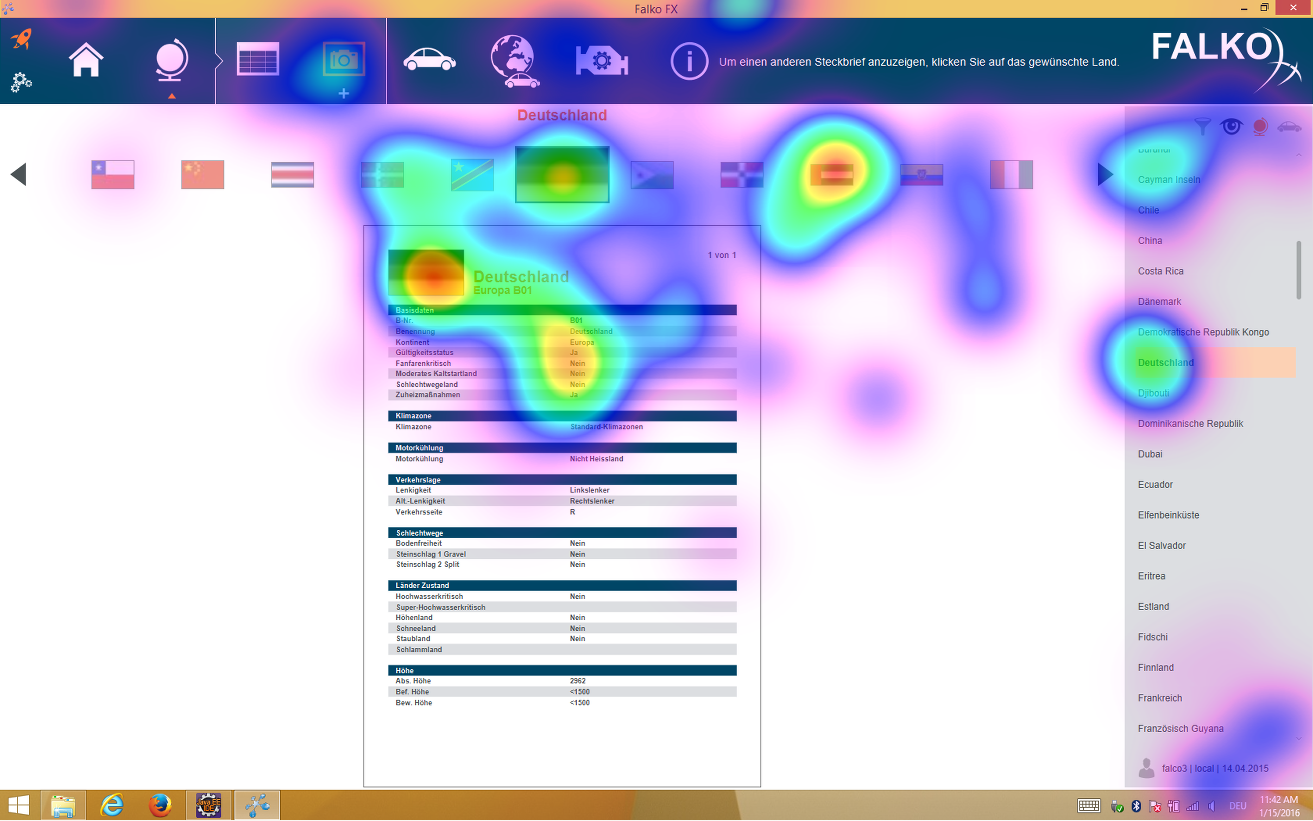
\includegraphics[width=0.6\textwidth]{grafiken/gallery_heatmap.png}
 \caption{Heatmap Galerie-Bildschirm}
 \label{fig:galleryHeatmap}
\end{figure}
Die Grafik zeigt deutlich, dass das aktuell selektierte Element unter den Vorschaubildern am stärksten wahrgenommen wird. In der Seitenleiste zieht das orange markierte Element, das ebenfalls der Selektion entspricht, einige Aufmerksamkeit auf sich. Es wird aber auch deutlich, dass der Hilfetext im oberen Bereich der Anwendung sehr wenig beachtet wird. Dieses Phänomen ist nicht nur bei der Galerieansicht zu verfolgen. Auch bei der Ausführung anderer Aufgaben, die andere Bildschirme involvieren, wird der Hilfetext größtenteils ignoriert.\par
Eine Analyse des Blickweges eine Kandidaten zeigt, dass er Schnellfilter der Multi-Level-Liste erst zu einem späteren Zeitpunkt aktiv wahrgenommen wird. Die vorliegende Auswertung nutzt nur die Fixierungen der Augen auf bestimmte Bildpunkte für das Erstellen des Pfades.\par
\begin{figure}[H]
 \centering
 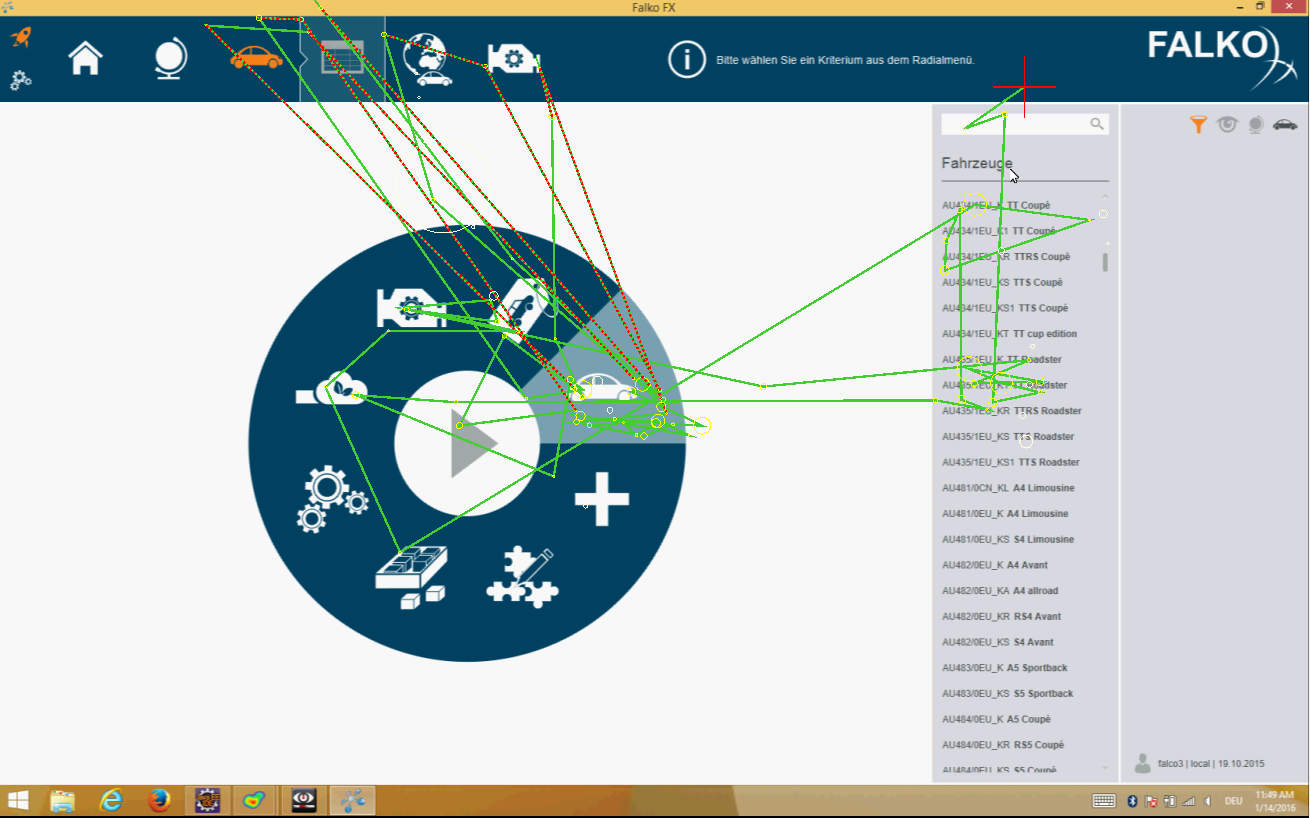
\includegraphics[width=0.6\textwidth]{grafiken/scanpath.png}
 \caption{Scanpath: Filter}
 \label{fig:scanFilter}
\end{figure}
Eine Areas Of Interest Analyse mit den Testdaten aller Kandidaten zeigt, dass der Bereich des Hilfetextes extrem selten/ kurz angeschaut wurde. Selbst das Logo hat mehr Aufmerksamkeit erhalten. Besonders im Fokus der Anwender standen auf dem Filterbildschirm die Multi-Level-Liste und die Seitenleiste. Das Radialmenü wurde vermehrt oben-/ rechtsseitig betrachtet. Viel Zeit wurde außerdem auf das Betrachten der Navigationsleiste aufgewandt.
\begin{figure}[H]
 \centering
 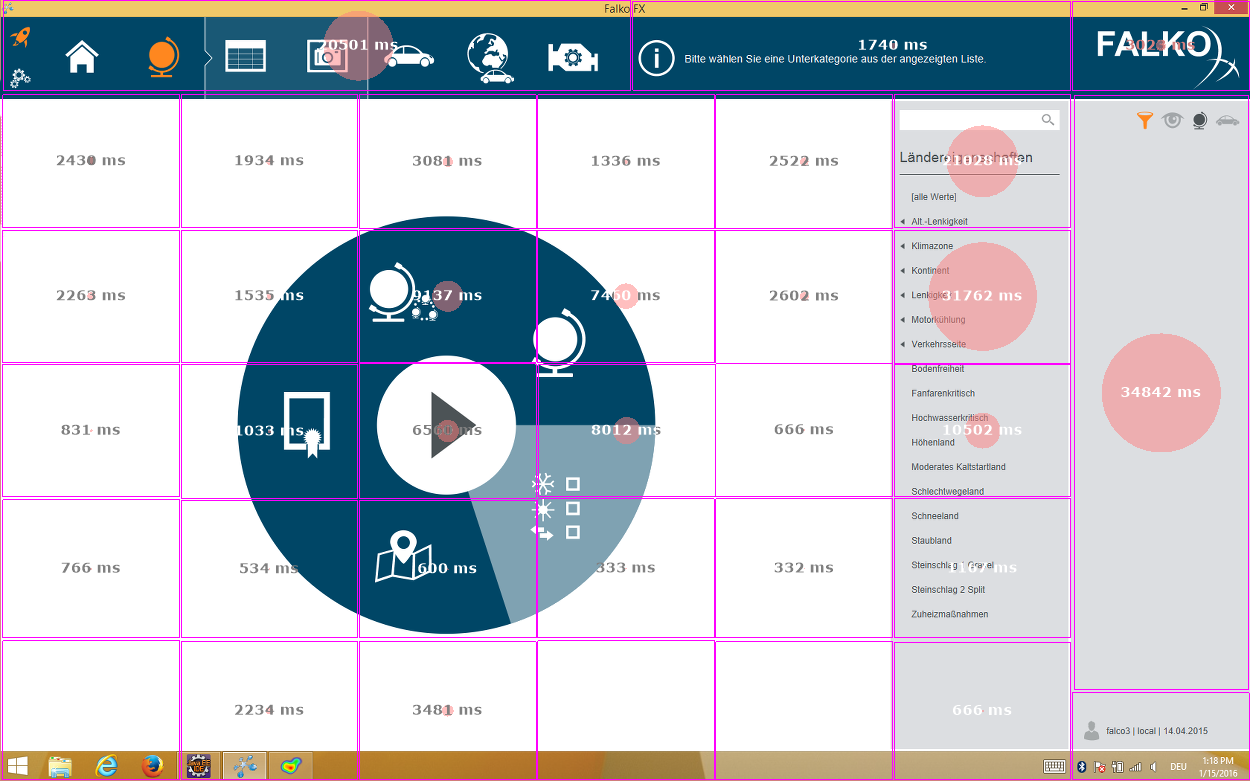
\includegraphics[width=0.7\textwidth]{grafiken/areas_of_interest_filter.png}
 \caption{Areas Of Interest: Filter}
 \label{fig:aoiFIlter}
\end{figure}
\heading{Usability-Befragung}
Die Usability-Befragung bietet nicht direkt Aufschluss darüber, an welchen Stellen Probleme vorhanden sein könnten. Stattdessen bietet sie Anhaltspunkte, in welchen Kategorien, aufgrund der subjektiven Wahrnehmung der Testkandidaten, mehr Aufwand für ein optimales Gesamtergebnis betrieben werden muss.\par
Die Umfrageergebnisse haben eine deutlich positive Tendenz. Vor allem die Attraktivität der Anwendung wurde durch die Testkandidaten hervorgehoben. Im Bereich der Pragmatischen Qualität muss aus Sicht der Testkandidaten allerdings noch mehr Aufwand betrieben werden. Dies lässt sich teilweise, aber nicht vollständig auf das fehlende Fachwissen zurückführen. Die Hedonische Qualität ergibt sich zum Teil aus den zahlreichen Bedienungsmöglichkeiten, die unter anderem im Rahmen dieser Arbeit umgesetzt wurden. Nutzer, die sich intensiver und häufiger mit der Anwendung beschäftigen, würden die Bereiche Eigenschaften der Anwendung auf eine andere Art und Weise wahrnehmen.\par
\editHere{word-pairs}
